% !TeX root = ../paper.tex
% !TeX encoding = UTF-8
% !TeX spellcheck = en_US

\section{Actor Memory Overhead Experiments}\label{sec:experiments}

  Our concept is based on the usage of hundreds of thousands of \glspl{dactor}, which all store only a small amount of data.
  This raises the question of how much memory overhead is introduced for storing data split across a multitude of actors.
  Therefore, we performed experiments comparing the memory usage of an exemplary actor database system with that of just loading the data into our data storage abstraction, called relations, or in a big string into memory.

\subsection{Experimental Setup}

  The exemplary actor database system used for testing consists of four different \gls{dactor} types, each containing different number of relations and data sizes.
  We used a script to generate four different datasets emulating the scaling of the system by increasing the number of \gls{dactor}-instances in the system and keeping the data size stored in one \gls{dactor} nearly constant.
  The script creates various primitive data types, such as \code{String}, \code{Double}, and \code{Int}, as well as complex data types, such as \code{ZonedDateTime}, and distributes the data across \glspl{dactor} and relations.
  The data distribution across the \gls{dactor} types is reported in table~\ref{tab:datasets:size_distribution} and the key figures of the datasets are reported in table~\ref{tab:datasets:keyfigures}.
  
  \begin{table}
    \centering
    \begin{subtable}[t]{0.445\textwidth}
      \centering
      \begin{tabular}{@{}crr@{}}
        \toprule
        \textbf{\gls{dactor} type} & \textbf{Data size} & \textbf{\# Relations}\\
        \midrule
        $X_1$ &   7~KB & 2 \\ % Cart
        $X_2$ &  22~KB & 3 \\ % Customer
        $X_3$ & 171~KB & 2 \\ % StoreSection
        $X_4$ & 721~KB & 1 \\ % GroupManager
        \bottomrule
      \end{tabular}
      \subcaption{\gls{dactor} types and their corresponding data sizes}
      \label{tab:datasets:size_distribution}
    \end{subtable}
    \begin{subtable}[t]{0.545\textwidth}
      \centering
      \begin{tabular}{@{}crrr@{}}
        \toprule
        \textbf{Dataset} & \textbf{Size on disk} & \textbf{\# \glspl{dactor}} & \textbf{\# Relations}\\
        \midrule
        $D_1$ & 10~MB & 829 & 1~714 \\
        $D_2$ & 25~MB & 2~578 & 5~250 \\
        $D_3$ & 50~MB & 4~373 & 8~935 \\
        $D_4$ & 100~MB & 8~618 & 17~596 \\
        \bottomrule
      \end{tabular}
      \subcaption{Datasets sizes and key figures}
      \label{tab:datasets:keyfigures}
    \end{subtable}
    \caption{Datasets used for the memory overhead experiments}
    \label{tab_datasets}
  \end{table}

  For each dataset we performed three different tests:
  \begin{description}
    \item[\textit{SingleString}] Convert all data into its \code{String} representation and load it as a single big \code{String} into memory.
      This test serves as baseline for the other ones.
    \item[\textit{Relations}] Load the data into their respective \code{Relation}s, preserving the type information and using the in-memory data storage objects from our framework.
    \item[\textit{Framework}] Use the full-fledged framework to load the data into memory.
      This approach stores the data distributed across \glspl{dactor} in \code{Relation} objects.
  \end{description}

  To obtain the used memory of the objects in our test approaches, we used VisualVM\footnote{\url{https://visualvm.github.io/}} to create heap dumps.
  After the data was completely loaded into memory, we triggered a garbage collection run and created a heap dump.
  VisualVM is able to compute the retained sizes of object hierarchies in those dumps.
  This allowed us to investigate the memory usage of selected objects and their members in detail.
  We report and discuss the results of those experiments in the next section.

\subsection{Results}

  \begin{figure}
    \centering
    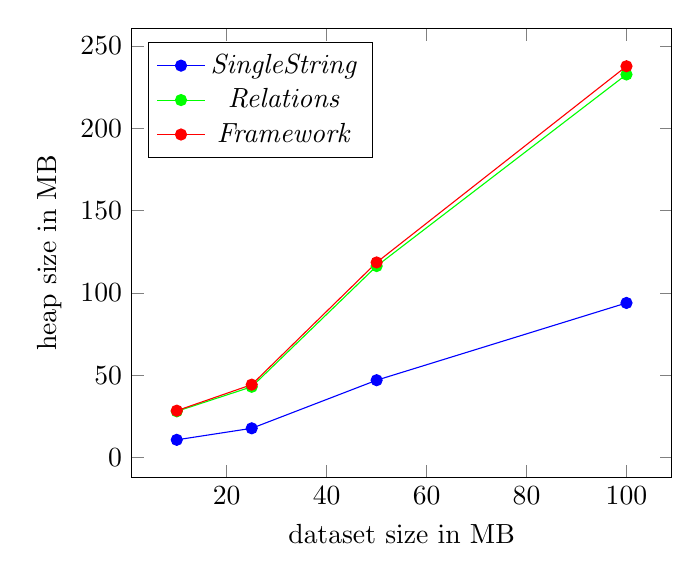
\begin{tikzpicture}
      \begin{axis}[
          xlabel=dataset size in MB, ylabel=heap size in MB,
          legend pos=north west
      ]
        \addplot[mark=*, color=blue] coordinates {
          (10,10.8)
          (25,17.8)
          (50,47.0)
          (100,93.9)
        };
        \addplot[mark=*, color=green] coordinates {
          (10,28.1)
          (25,43.0)
          (50,116.3)
          (100,232.6)
        };
        \addplot[mark=*, color=red] coordinates {
          (10,28.5)
          (25,44.3)
          (50,118.5)
          (100,237.6)
        };
      
      \legend{\textit{SingleString}, \textit{Relations}, \textit{Framework}}
      \end{axis}
    \end{tikzpicture}
    \caption{Used heap size when loading the data into memory using the three different methods.}
    \label{fig:exp:general}
  \end{figure}

  \begin{figure}
    \centering
    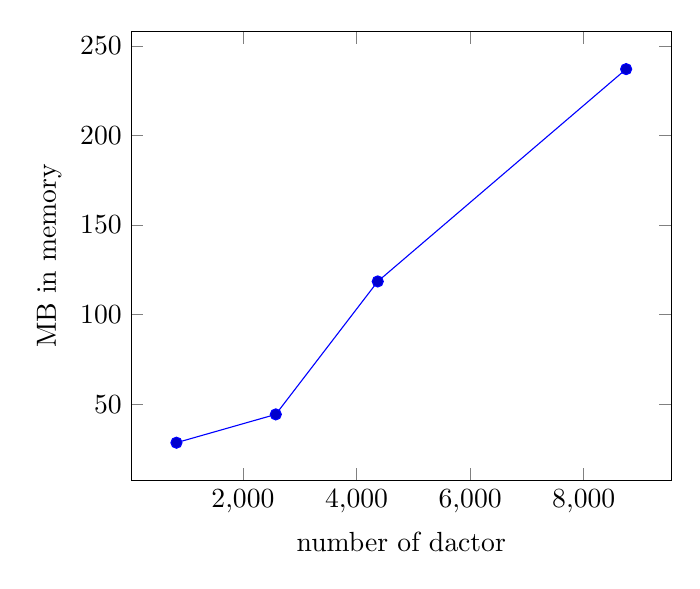
\begin{tikzpicture}
      \begin{axis}[xlabel=number of \glspl{dactor},ylabel=MB in memory]
        \addplot coordinates {
          (829,28.5)
          (2578,44.3)
          (4373,118.5)
          (8746,237.0)
        };
      \end{axis}
    \end{tikzpicture}
    \caption{Memory consumption as a function of the number of \glspl{dactor}}
    \label{fig:exp:dactors}
  \end{figure}


  \begin{figure}
    \centering
    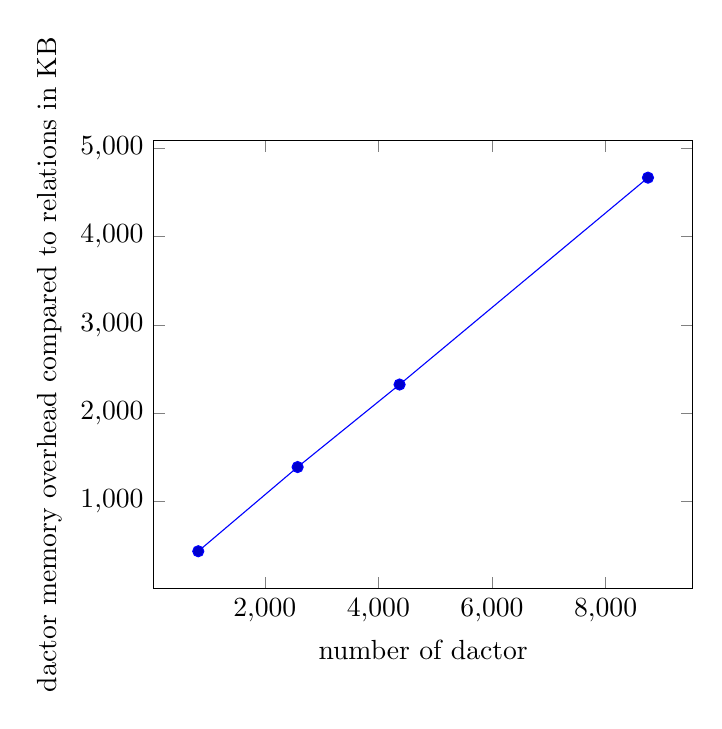
\begin{tikzpicture}
      \begin{axis}[xlabel=number of \glspl{dactor},ylabel=\gls{dactor} memory overhead compared to relations in KB]
        \addplot coordinates {
          (829,436)   % ratio: 0.526
          (2578,1390) % ratio: 0.539
          (4373,2325) % ratio: 0.532
          (8746,4669) % ratio: 0.534
        };
      \end{axis}
    \end{tikzpicture}
    \caption{Memory overhead of \glspl{dactor} as a function of the number of \glspl{dactor}}
    \label{fig:exp:dactoroverhead}
  \end{figure}

  \begin{figure}
    \centering
    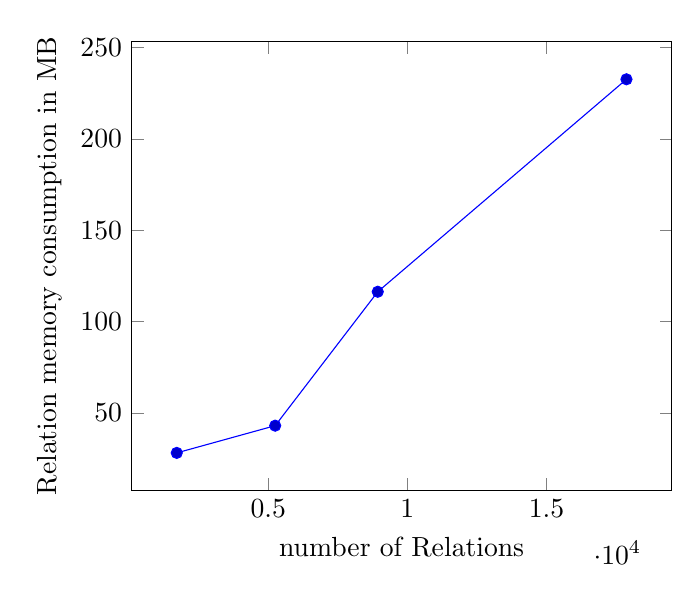
\begin{tikzpicture}
      \begin{axis}[xlabel=number of Relations,ylabel=Relation memory consumption in MB]
        \addplot coordinates {
          (1714,28.1)
          (5250,43.0)
          (8935,116.3)
          (17870,232.6)
        };
      \end{axis}
    \end{tikzpicture}
    \caption{Memory overhead of Relations as a function of the number of Relations}
    \label{fig:exp:relationoverhead}
  \end{figure}

\subsection{Discussion}
